\chapter{Pola Arsitektur Aplikasi Web: MVC dan ExpressJS}

\section{Apa itu Pola Arsitektur?}

\index{Pola arsitektur}Pola arsitektur (\textit{architectural pattern}) adalah konsep dan standar arsitektur yang membentuk suatu aplikasi. Pola disini mengacu pada \textit{best practices} atau praktik-praktik terbaik yang terutama terkait dengan arsitektur dari software aplikasi. Pola arsitektur terdiri atas elemen-elemen software, properti dari elemen-elemen tersebut, serta hubungan antar elemen-elemen tersebut.

\section{Pola Arsitektur MVC}

\index{MVC}MVC (Model-View-Controller) merupakan pola arsitektur aplikasi Web yang memisahkan aplikasi Web menjadi 3 komponen:
\begin{itemize}
	\item Model: basis data
	\item View: tampilan antarmuka aplikasi Web, biasanya berisi semacam template dan isi-isi dinamis dari tampilan antarmuka tersebut.
	\item Controller: menerima \textit{requests} atau permintaan dari browser kemudian mengarahkan ke \textit{event-handler} untuk diproses. Proses tersebut bisa saja berupa langsung menghasilkan view (X)HTML atau format lainnya, atau bisa juga diproses terlebih dahulu di model dan kemudian hasilnya akan dikirimkan ke view untuk diisikan ke isi-isi dinamis serta membentuk file (X)HTML untuk ditampilkan di browser (sebenarnya tidak selalu perlu harus (X)HTML).
\end{itemize}

Jika digambarkan dalam suatu diagram, pola arsitektur MVC ditampilkan pada gambar~\ref{fig:mvc}

  \begin{figure}
    \begin{center}
      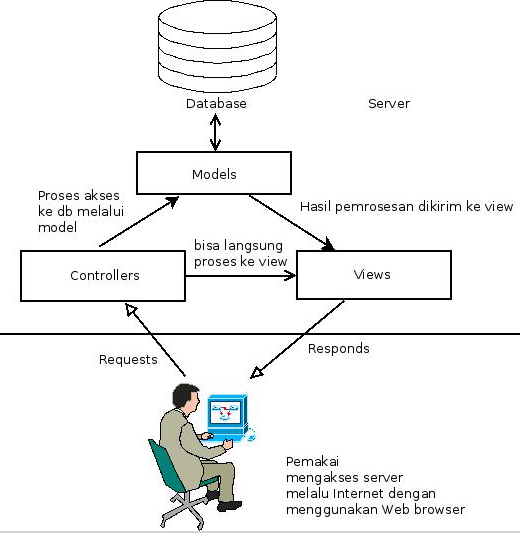
\includegraphics[scale=0.5]{images/mvc.jpg}
    \end{center}
    \caption{Pola arsitektur MVC}
    \label{fig:mvc}
  \end{figure}

Pola ini dikenal juga dengan istilah Model 2 dan dipopulerkan oleh JavaEE. 

\section{Implementasi Pola Arsitektur MVC Menggunakan ExpressJS}

\index{MVC!dan ExpressJS}Sebenarnya ExpressJS bukan merupakan \textit{framework} MVC, meskipun demikian karena framework ini sangat fleksibel, maka pemrogram bisa mengatur sendiri lokasi dari file / direktori serta berbagai konfigurasi lainnya. Contoh implementasi disini adalah aplikasi sederhana untuk menampilkan data yang tersimpan dalam basis data mongoDB ke dalam format JSON yang bisa diakses dari browser.

\subsection{Struktur Aplikasi}

Setelah membuat kerangka aplikasi menggunakan ExpressJS, ada beberapa perubahan yang harus dilakukan. Perubahan ini terutama dilakukan untuk mengikuti pola arsitektur MVC (terutama peletakan file dan direktori). Pola asli dari kerangka aplikasi ExpressJS adalah sebagai berikut:

\lstset{language=Bash,caption=Struktur direktori asli aplikasi ExpressJS}
\begin{lstlisting}
$ tree .
.
+-- app.js
|-- package.json
|-- public
|   +-- images
|   |-- javascripts
|   +-- stylesheets
|       +-- style.css
|-- routes
|   +-- index.js
|   +-- user.js
+-- views
    +-- index.jade
    +-- layout.jade

6 directories, 7 files
\end{lstlisting}

Struktur direktori tersebut akan diubah sesuai dengan pola MVC:

\lstset{language=Bash,caption=Struktur direktori ExpressJS sesuai pola MVC}
\begin{lstlisting}
$ tree .
.
+-- app.js
|-- controllers
|   +-- index.js
|   +-- user.js
|-- models
|   +-- db.js
|-- package.json
|-- public
|   +-- images
|   |-- javascripts
|   +-- stylesheets
|       +-- style.css
+-- views
    +-- index.jade
    +-- layout.jade

7 directories, 8 files
\end{lstlisting}

Beberapa perubahan terhadap struktur direktori:
\begin{itemize}
	\item direktori routes diubah menjadi \textit{controllers}
	\item membuat direktori \textit{models} untuk mendefinisikan skema basis data
\end{itemize}

\subsection{File-file yang Diperlukan}

Beberapa file diubah isinya dan ada juga file yang baru. 

\lstset{language=JavaScript,caption=app.js}
\begin{lstlisting}
/**
 * Module dependencies.
 */

var express = require('express')
  , controllers = require('./controllers')
  , user = require('./controllers/user')
  , http = require('http')
  , path = require('path');

var mongoose = require('mongoose');

var app = express();

mongoose.connect('mongodb://localhost/mydb');

app.configure(function(){
  app.set('port', process.env.PORT || 3000);
  app.set('views', __dirname + '/views');
  app.set('view engine', 'jade');
  app.use(express.favicon());
  app.use(express.logger('dev'));
  app.use(express.bodyParser());
  app.use(express.methodOverride());
  app.use(app.router);
  app.use(express.static(path.join(__dirname, 'public')));
});

app.configure('development', function(){
  app.use(express.errorHandler());
});

app.get('/', controllers.index);
app.get('/users', user.list);

http.createServer(app).listen(app.get('port'), function(){
  console.log("Express server listening on port " + app.get('port'));
});
\end{lstlisting}

\lstset{language=JavaScript,caption=controllers/user.js}
\begin{lstlisting}
/*
 * GET employees listing.
 */

var Employee = require('../models/db.js');

exports.list = function(req, res){
	Employee.find(function(err, employees) {
	  res.send(employees);
	});
};
\end{lstlisting}

\lstset{language=JavaScript,caption=models/db.js}
\begin{lstlisting}
var mongoose = require('mongoose')
   ,Schema = mongoose.Schema;
 
var employeeSchema = new Schema({
    name: String,
		address: String,
    phone: String,
    email: String
});
 
module.exports = mongoose.model('Employee', employeeSchema);
\end{lstlisting}


\lstset{language=JavaScript,caption=package.json}
\begin{lstlisting}
{
  "name": "express-mvc",
  "version": "0.0.1",
  "private": true,
  "scripts": {
    "start": "node app"
  },
  "dependencies": {
    "express": "latest",
    "jade": "*",
    "mongoose": "latest"
  }
}
\end{lstlisting}

\subsection{Hasil}

Setelah server dieksekusi (menggunakan perintah \textit{node app.js}), maka hasilnya akan bisa diakses di \url{http://localhost:3000/users}. Hasil di browser bisa dilihat di gambar~\ref{fig:hasil-mvc}

  \begin{figure}
    \begin{center}
      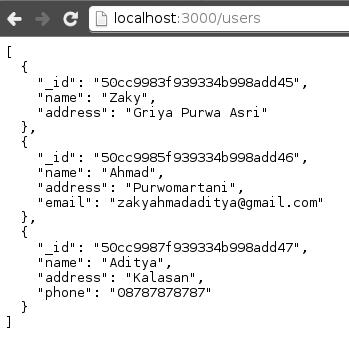
\includegraphics[scale=0.5]{images/mvc-result.jpg}
    \end{center}
    \caption{Pola arsitektur MVC}
    \label{fig:hasil-mvc}
  \end{figure}

\section{Pola Arsitektur Aplikasi Web Lain dan Implementasinya}

MVC bukan satu-satu pola arsitektur aplikasi Web. Berikut ini adalah beberapa daftar pola arsitektur aplikasi Web serta implementasinya di Node.js dan/atau JavaScript di sisi klien:
\begin{itemize}
\item MVP (Model-View-Presenter): Google GWT.
\item MVVM (Model-View-ViewModel): Batman.js (\url{http://batmanjs.org}) dan Knockout.js (\url{http://knockoutjs.com})
\item RVP (Resource-View-Presenter): Flatiron (\url{http://flatironjs.org})
\item MVA (Model-View-Adapter).
\item Hierarchical MVC
\item Presentation-Abstract-Control.
\end{itemize}
